\subsection{U.S. CBP Regressions}
The following are regressions of log dentist office (NAICS 6211--) employment per capita in U.S. border counties against different control groups.
Demographic variables are included as controls.

\begin{table}[H]
	\caption{Control: Canada Border Counties}
	\centering
{
\def\sym#1{\ifmmode^{#1}\else\(^{#1}\)\fi}
\begin{tabular}{l*{6}{c}}
\toprule
                    &\multicolumn{1}{c}{(1)}         &\multicolumn{1}{c}{(2)}         &\multicolumn{1}{c}{(3)}         &\multicolumn{1}{c}{(4)}         &\multicolumn{1}{c}{(5)}         &\multicolumn{1}{c}{(6)}         \\
\midrule
Borders Mexico      &      -0.334\sym{*}  &      -0.303         &      -0.267         &      -0.365         &      -0.436\sym{*}  &       0.204         \\
                    &     (0.143)         &     (0.162)         &     (0.170)         &     (0.209)         &     (0.213)         &     (0.436)         \\
\addlinespace
Log Population      &                     &       0.120         &       0.117         &       0.131         &       0.154         &      0.0926         \\
                    &                     &     (0.105)         &     (0.105)         &     (0.108)         &     (0.108)         &     (0.114)         \\
\addlinespace
Log Pop. Density    &                     &     -0.0346         &     -0.0165         &     -0.0496         &     -0.0430         &   -0.000770         \\
                    &                     &    (0.0836)         &    (0.0876)         &    (0.0902)         &    (0.0892)         &    (0.0946)         \\
\addlinespace
Log Median. HH Income&                     &       1.027\sym{**} &       1.185\sym{**} &       0.999\sym{**} &       1.327\sym{**} &       1.016\sym{*}  \\
                    &                     &     (0.336)         &     (0.400)         &     (0.345)         &     (0.412)         &     (0.453)         \\
\addlinespace
Proportion 25-54    &                     &                     &      -4.365         &                     &      -11.15         &      -11.92         \\
                    &                     &                     &     (5.934)         &                     &     (7.869)         &     (7.804)         \\
\addlinespace
Proportion 55+      &                     &                     &                     &      -1.213         &      -4.403         &      -8.401\sym{*}  \\
                    &                     &                     &                     &     (2.566)         &     (3.389)         &     (4.122)         \\
\addlinespace
Proportion Black    &                     &                     &                     &                     &                     &      -0.339         \\
                    &                     &                     &                     &                     &                     &     (1.298)         \\
\addlinespace
Proportion Hispanic &                     &                     &                     &                     &                     &      -1.215         \\
                    &                     &                     &                     &                     &                     &     (0.729)         \\
\midrule
N                   &          46         &          46         &          46         &          46         &          46         &          46         \\
Mean                &      .00108         &      .00108         &      .00108         &      .00108         &      .00108         &      .00108         \\
State FE            &          No         &          No         &          No         &          No         &          No         &          No         \\
\bottomrule
\multicolumn{7}{l}{\footnotesize Standard errors in parentheses. Mean refers to original (non-logged) outcome variable.}\\
\multicolumn{7}{l}{\footnotesize * p<0.05, ** p<0.01, *** p<0.001}\\
\end{tabular}
}

\end{table}

\begin{table}[H]
	\caption{Control: Adjacent U.S. Counties}
	\centering
{
\def\sym#1{\ifmmode^{#1}\else\(^{#1}\)\fi}
\begin{tabular}{l*{6}{c}}
\toprule
                    &\multicolumn{1}{c}{(1)}         &\multicolumn{1}{c}{(2)}         &\multicolumn{1}{c}{(3)}         &\multicolumn{1}{c}{(4)}         &\multicolumn{1}{c}{(5)}         &\multicolumn{1}{c}{(6)}         \\
\midrule
Borders Mexico      &      -0.135         &      -0.117         &     -0.0842         &     -0.0585         &     -0.0792         &       0.169         \\
                    &     (-0.66)         &     (-0.55)         &     (-0.39)         &     (-0.26)         &     (-0.33)         &      (0.87)         \\
\addlinespace
Log Population      &                     &      0.0883         &       0.112         &       0.104         &       0.112         &       0.117         \\
                    &                     &      (0.54)         &      (0.67)         &      (0.62)         &      (0.65)         &      (0.61)         \\
\addlinespace
Log Pop. Density    &                     &      0.0521         &      0.0320         &      0.0419         &      0.0329         &      0.0309         \\
                    &                     &      (0.37)         &      (0.22)         &      (0.29)         &      (0.22)         &      (0.20)         \\
\addlinespace
Log Median. HH Income&                     &       0.654         &       1.007         &       0.767         &       0.981         &       0.229         \\
                    &                     &      (1.00)         &      (1.30)         &      (1.14)         &      (1.07)         &      (0.31)         \\
\addlinespace
Proportion 25-54    &                     &                     &      -6.064         &                     &      -5.310         &      -13.11         \\
                    &                     &                     &     (-0.87)         &                     &     (-0.35)         &     (-0.85)         \\
\addlinespace
Proportion 55+      &                     &                     &                     &       2.449         &       0.382         &      -8.692         \\
                    &                     &                     &                     &      (0.79)         &      (0.06)         &     (-1.21)         \\
\addlinespace
Proportion Black    &                     &                     &                     &                     &                     &      -4.814         \\
                    &                     &                     &                     &                     &                     &     (-0.75)         \\
\addlinespace
Proportion Hispanic &                     &                     &                     &                     &                     &      -2.812\sym{**} \\
                    &                     &                     &                     &                     &                     &     (-3.61)         \\
\addlinespace
Constant            &      -6.988\sym{***}&      -15.59\sym{*}  &      -18.59\sym{*}  &      -17.37\sym{*}  &      -18.49\sym{*}  &      -5.771         \\
                    &    (-44.75)         &     (-2.39)         &     (-2.50)         &     (-2.49)         &     (-2.36)         &     (-0.84)         \\
\midrule
N                   &          25         &          25         &          25         &          25         &          25         &          25         \\
State FE            &         Yes         &         Yes         &         Yes         &         Yes         &         Yes         &         Yes         \\
\bottomrule
\multicolumn{7}{l}{\footnotesize \textit{t} statistics in parentheses}\\
\multicolumn{7}{l}{\footnotesize \sym{*} \(p<0.05\), \sym{**} \(p<0.01\), \sym{***} \(p<0.001\)}\\
\end{tabular}
}

\end{table}

\begin{table}[H]
	\caption{Control: Counties Within Five Adjacencies}
	\centering
{
\def\sym#1{\ifmmode^{#1}\else\(^{#1}\)\fi}
\begin{tabular}{l*{6}{c}}
\toprule
                    &\multicolumn{1}{c}{(1)}         &\multicolumn{1}{c}{(2)}         &\multicolumn{1}{c}{(3)}         &\multicolumn{1}{c}{(4)}         &\multicolumn{1}{c}{(5)}         &\multicolumn{1}{c}{(6)}         \\
\midrule
Borders Mexico      &      -0.173         &      -0.191         &      -0.178         &      -0.125         &      -0.164         &     -0.0625         \\
                    &     (0.144)         &     (0.131)         &     (0.126)         &     (0.129)         &     (0.131)         &     (0.148)         \\
\addlinespace
Log Population      &                     &      0.0672         &       0.117         &       0.121         &       0.122         &       0.131\sym{*}  \\
                    &                     &    (0.0619)         &    (0.0616)         &    (0.0630)         &    (0.0627)         &    (0.0628)         \\
\addlinespace
Log Pop. Density    &                     &      0.0951         &      0.0760         &      0.0631         &      0.0715         &      0.0835         \\
                    &                     &    (0.0606)         &    (0.0587)         &    (0.0599)         &    (0.0599)         &    (0.0590)         \\
\addlinespace
Log Median. HH Income&                     &       0.614\sym{**} &       0.803\sym{***}&       0.638\sym{**} &       0.774\sym{***}&       0.592\sym{*}  \\
                    &                     &     (0.210)         &     (0.210)         &     (0.204)         &     (0.223)         &     (0.229)         \\
\addlinespace
Proportion 25-54    &                     &                     &      -7.094\sym{**} &                     &      -5.772         &      -4.927         \\
                    &                     &                     &     (2.192)         &                     &     (3.894)         &     (4.136)         \\
\addlinespace
Proportion 55+      &                     &                     &                     &       3.072\sym{**} &       0.773         &      -0.782         \\
                    &                     &                     &                     &     (1.067)         &     (1.879)         &     (2.041)         \\
\addlinespace
Proportion Black    &                     &                     &                     &                     &                     &      -2.438         \\
                    &                     &                     &                     &                     &                     &     (1.729)         \\
\addlinespace
Proportion Hispanic &                     &                     &                     &                     &                     &      -0.674\sym{*}  \\
                    &                     &                     &                     &                     &                     &     (0.285)         \\
\midrule
N                   &         131         &         131         &         131         &         131         &         131         &         131         \\
Mean                &      .00117         &      .00117         &      .00117         &      .00117         &      .00117         &      .00117         \\
State FE            &         Yes         &         Yes         &         Yes         &         Yes         &         Yes         &         Yes         \\
\bottomrule
\multicolumn{7}{l}{\footnotesize Standard errors in parentheses. Mean refers to original (non-logged) outcome variable.}\\
\multicolumn{7}{l}{\footnotesize * p<0.05, ** p<0.01, *** p<0.001}\\
\end{tabular}
}

\end{table}

\begin{table}[H]
	\caption{Control: Counties Within Five Adjacencies (Dummies)}
	\centering
{
\def\sym#1{\ifmmode^{#1}\else\(^{#1}\)\fi}
\begin{tabular}{l*{6}{c}}
\toprule
                    &\multicolumn{1}{c}{(1)}         &\multicolumn{1}{c}{(2)}         &\multicolumn{1}{c}{(3)}         &\multicolumn{1}{c}{(4)}         &\multicolumn{1}{c}{(5)}         &\multicolumn{1}{c}{(6)}         \\
\midrule
Counties from Border=0&      -0.165         &      -0.191         &      -0.213         &      -0.156         &      -0.200         &     -0.0709         \\
                    &     (0.171)         &     (0.164)         &     (0.158)         &     (0.159)         &     (0.161)         &     (0.187)         \\
\addlinespace
Counties from Border=1&    -0.00409         &     -0.0500         &     -0.0667         &     -0.0785         &     -0.0709         &      0.0188         \\
                    &     (0.203)         &     (0.178)         &     (0.171)         &     (0.173)         &     (0.172)         &     (0.175)         \\
\addlinespace
Counties from Border=2&      -0.104         &     -0.0244         &     -0.0946         &     -0.0799         &     -0.0957         &     -0.0414         \\
                    &     (0.168)         &     (0.153)         &     (0.149)         &     (0.150)         &     (0.149)         &     (0.152)         \\
\addlinespace
Counties from Border=3&       0.123         &      0.0263         &      0.0127         &      0.0148         &      0.0123         &      0.0117         \\
                    &     (0.144)         &     (0.128)         &     (0.124)         &     (0.125)         &     (0.124)         &     (0.122)         \\
\addlinespace
Counties from Border=4&      0.0394         &      0.0589         &    0.000968         &     0.00440         &    -0.00214         &      0.0333         \\
                    &     (0.127)         &     (0.108)         &     (0.106)         &     (0.107)         &     (0.106)         &     (0.105)         \\
\addlinespace
Log Population      &                     &      0.0716         &       0.130         &       0.133         &       0.135         &       0.135         \\
                    &                     &    (0.0689)         &    (0.0689)         &    (0.0704)         &    (0.0700)         &    (0.0714)         \\
\addlinespace
Log Pop. Density    &                     &      0.0924         &      0.0651         &      0.0531         &      0.0601         &      0.0808         \\
                    &                     &    (0.0650)         &    (0.0632)         &    (0.0647)         &    (0.0645)         &    (0.0645)         \\
\addlinespace
Log Median. HH Income&                     &       0.602\sym{**} &       0.787\sym{***}&       0.621\sym{**} &       0.757\sym{**} &       0.578\sym{*}  \\
                    &                     &     (0.215)         &     (0.215)         &     (0.209)         &     (0.227)         &     (0.234)         \\
\addlinespace
Proportion 25-54    &                     &                     &      -7.263\sym{**} &                     &      -5.906         &      -4.885         \\
                    &                     &                     &     (2.275)         &                     &     (3.971)         &     (4.229)         \\
\addlinespace
Proportion 55+      &                     &                     &                     &       3.128\sym{**} &       0.799         &      -0.788         \\
                    &                     &                     &                     &     (1.106)         &     (1.914)         &     (2.114)         \\
\addlinespace
Proportion Black    &                     &                     &                     &                     &                     &      -2.586         \\
                    &                     &                     &                     &                     &                     &     (1.785)         \\
\addlinespace
Proportion Hispanic &                     &                     &                     &                     &                     &      -0.663\sym{*}  \\
                    &                     &                     &                     &                     &                     &     (0.306)         \\
\midrule
N                   &         131         &         131         &         131         &         131         &         131         &         131         \\
Mean                &      .00117         &      .00117         &      .00117         &      .00117         &      .00117         &      .00117         \\
State FE            &         Yes         &         Yes         &         Yes         &         Yes         &         Yes         &         Yes         \\
\bottomrule
\multicolumn{7}{l}{\footnotesize Standard errors in parentheses. Mean refers to original (non-logged) outcome variable.}\\
\multicolumn{7}{l}{\footnotesize * p<0.05, ** p<0.01, *** p<0.001}\\
\end{tabular}
}

\end{table}

\subsection{U.S. CBP Maps}
The following are county-level maps for counties in states along the Mexican border for dentist office employment per capita and ambulatory health services (NAICS 621---) employment per capita.
Note the censoring of sparsely-populated counties, especially in Texas.

\begin{figure}[H]
	\centering
	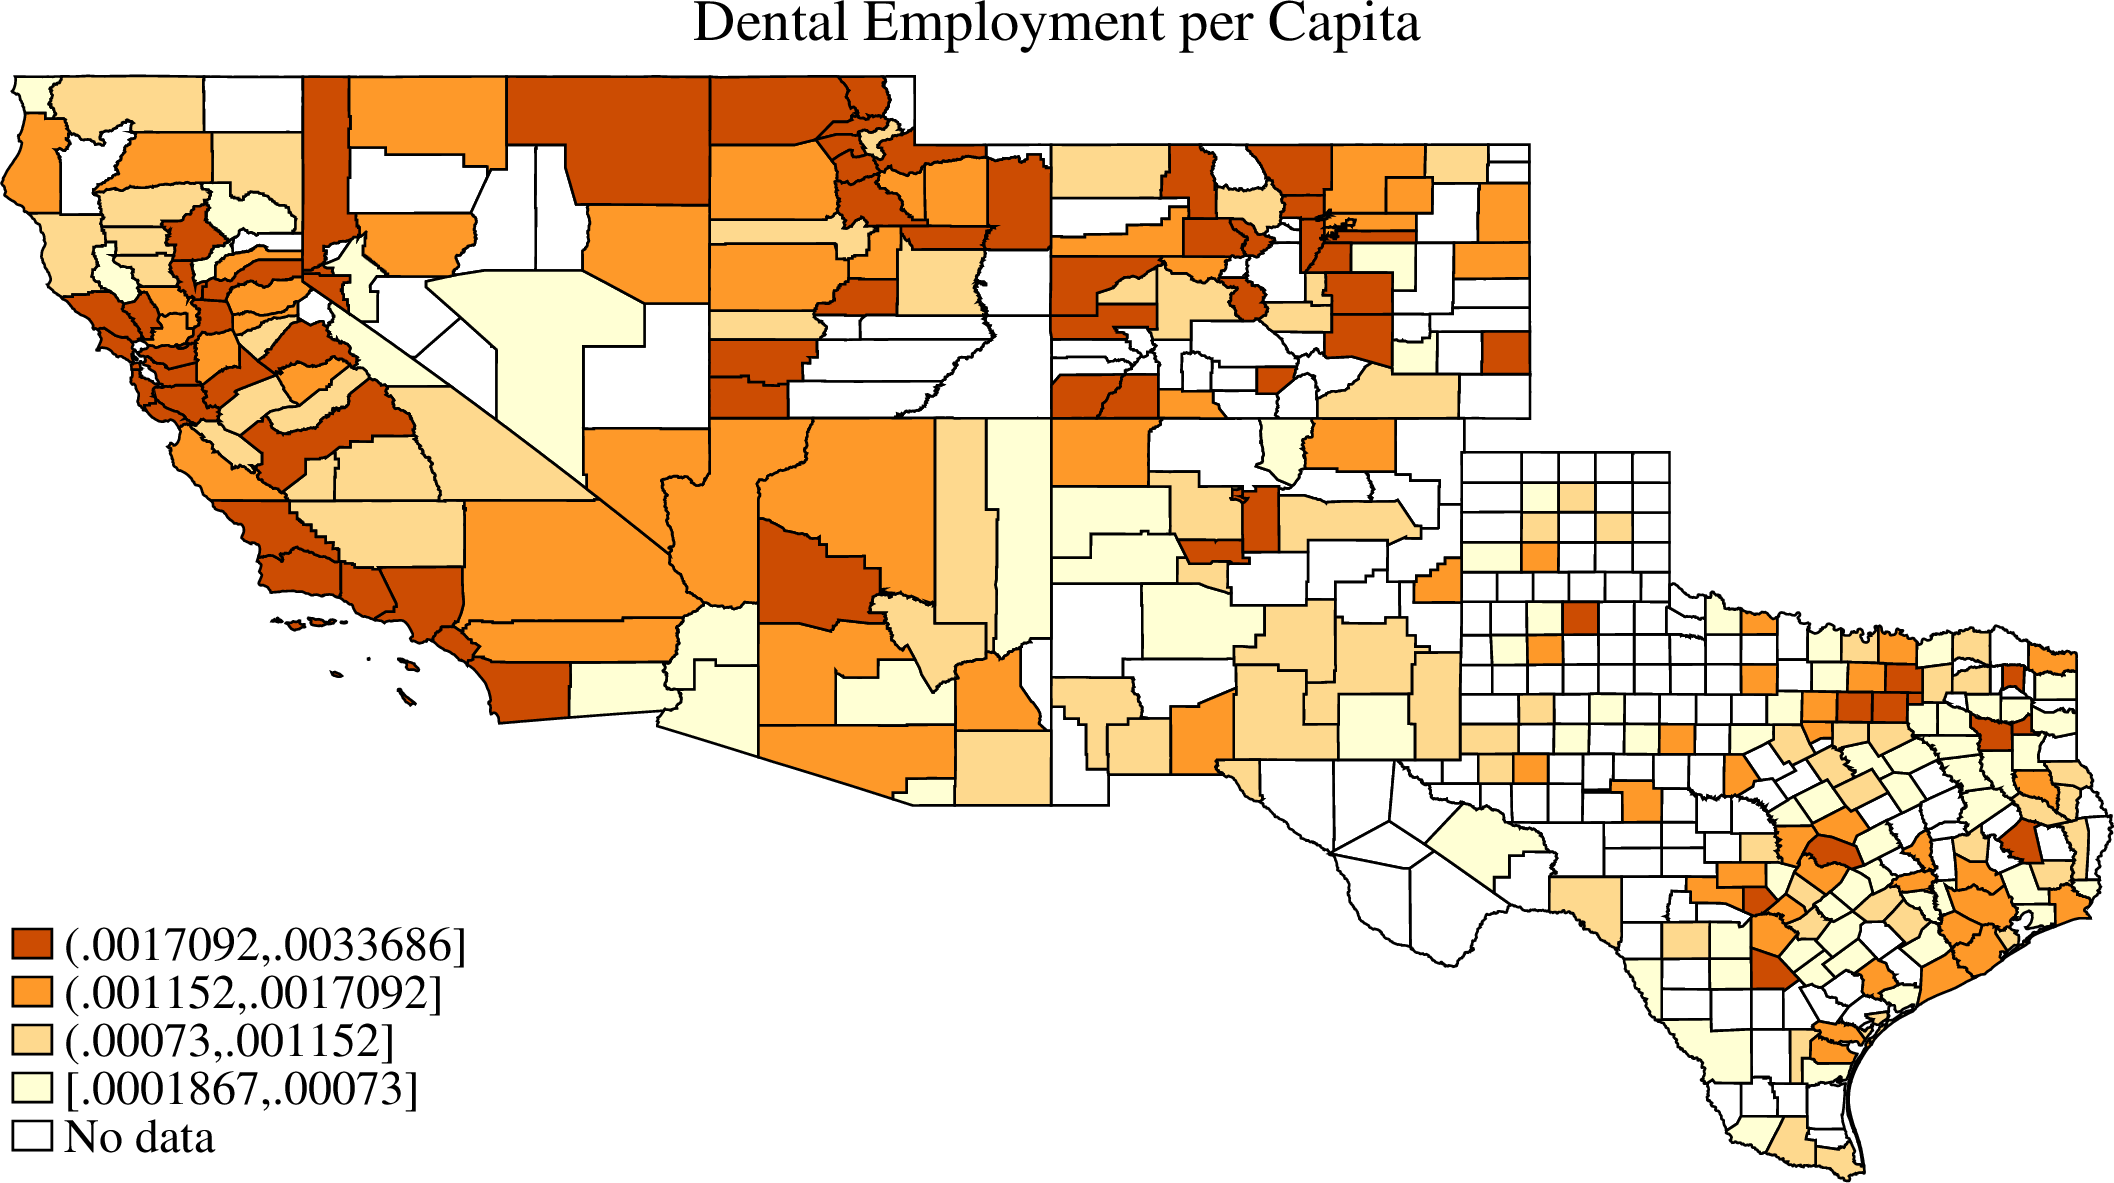
\includegraphics[width=.8\textwidth]{input/dentists_emp_pc_border.png}
\end{figure}

\begin{figure}[H]
	\centering
	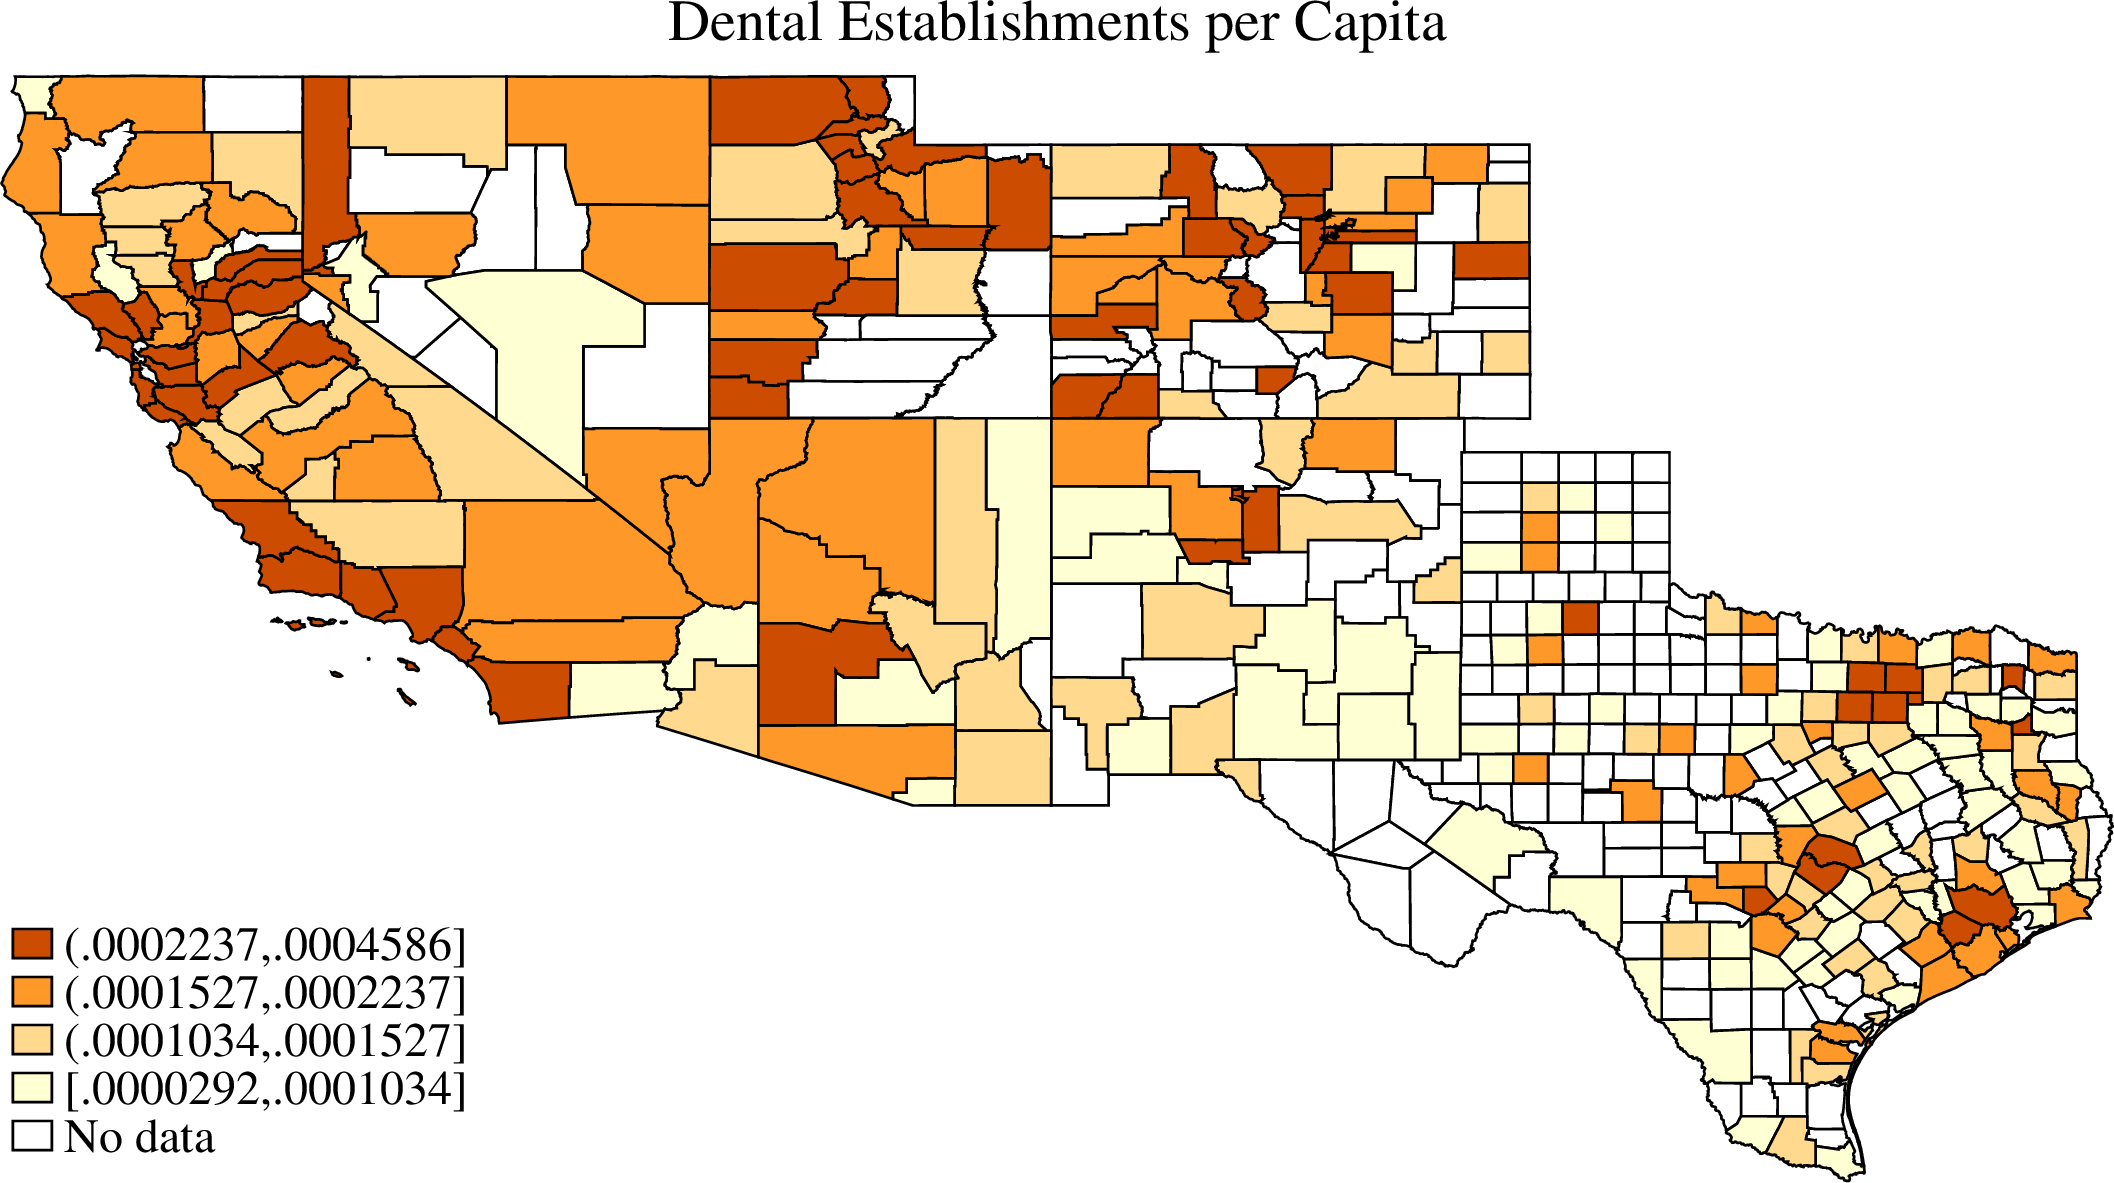
\includegraphics[width=.8\textwidth]{input/dentists_estabs_pc_border.png}
\end{figure}

\begin{figure}[H]
	\centering
	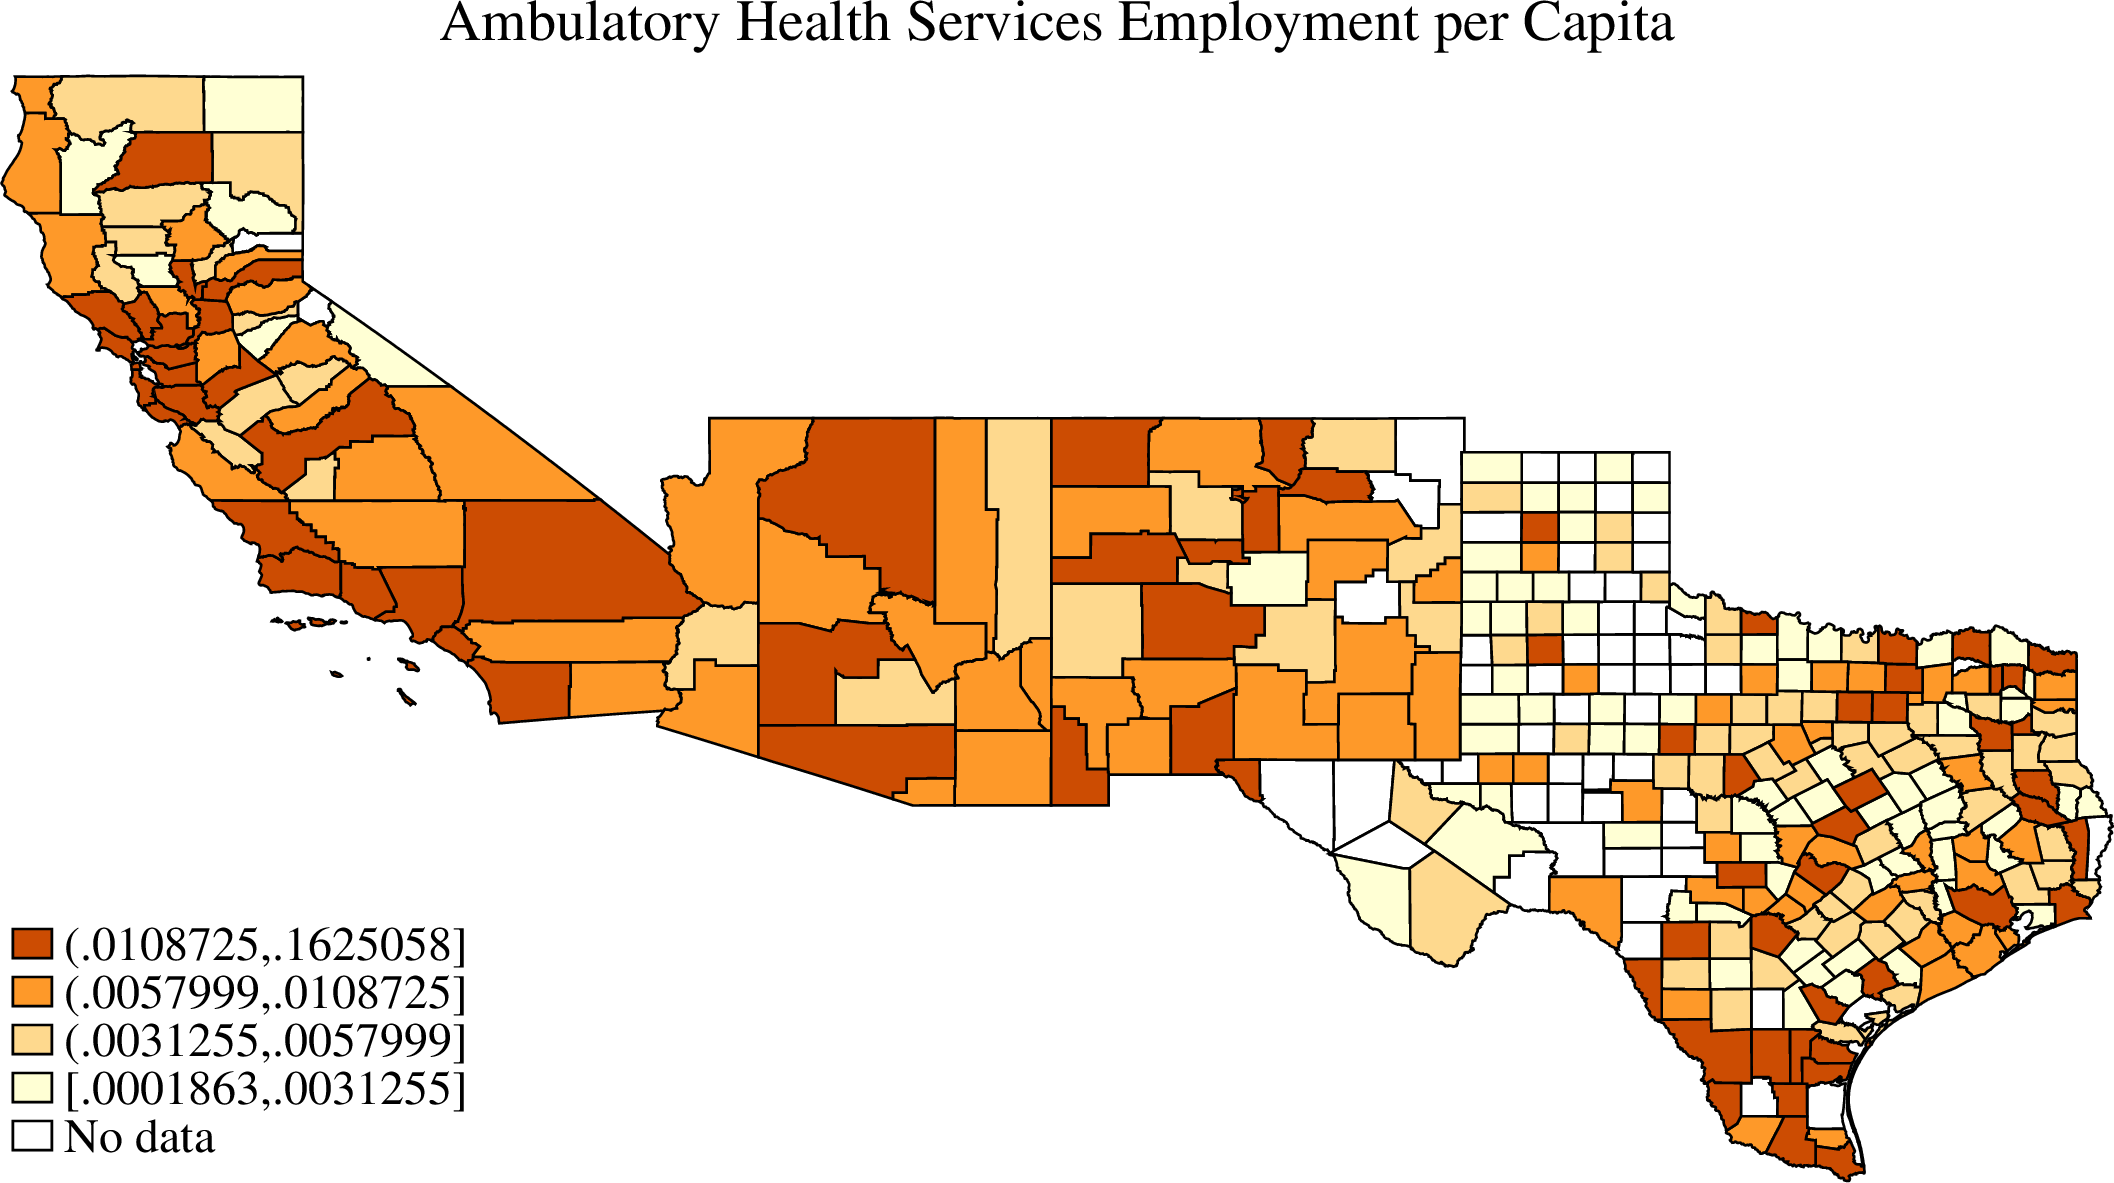
\includegraphics[width=.8\textwidth]{input/amb_health_services_emp_pc_border.png}
\end{figure}

\begin{figure}[H]
	\centering
	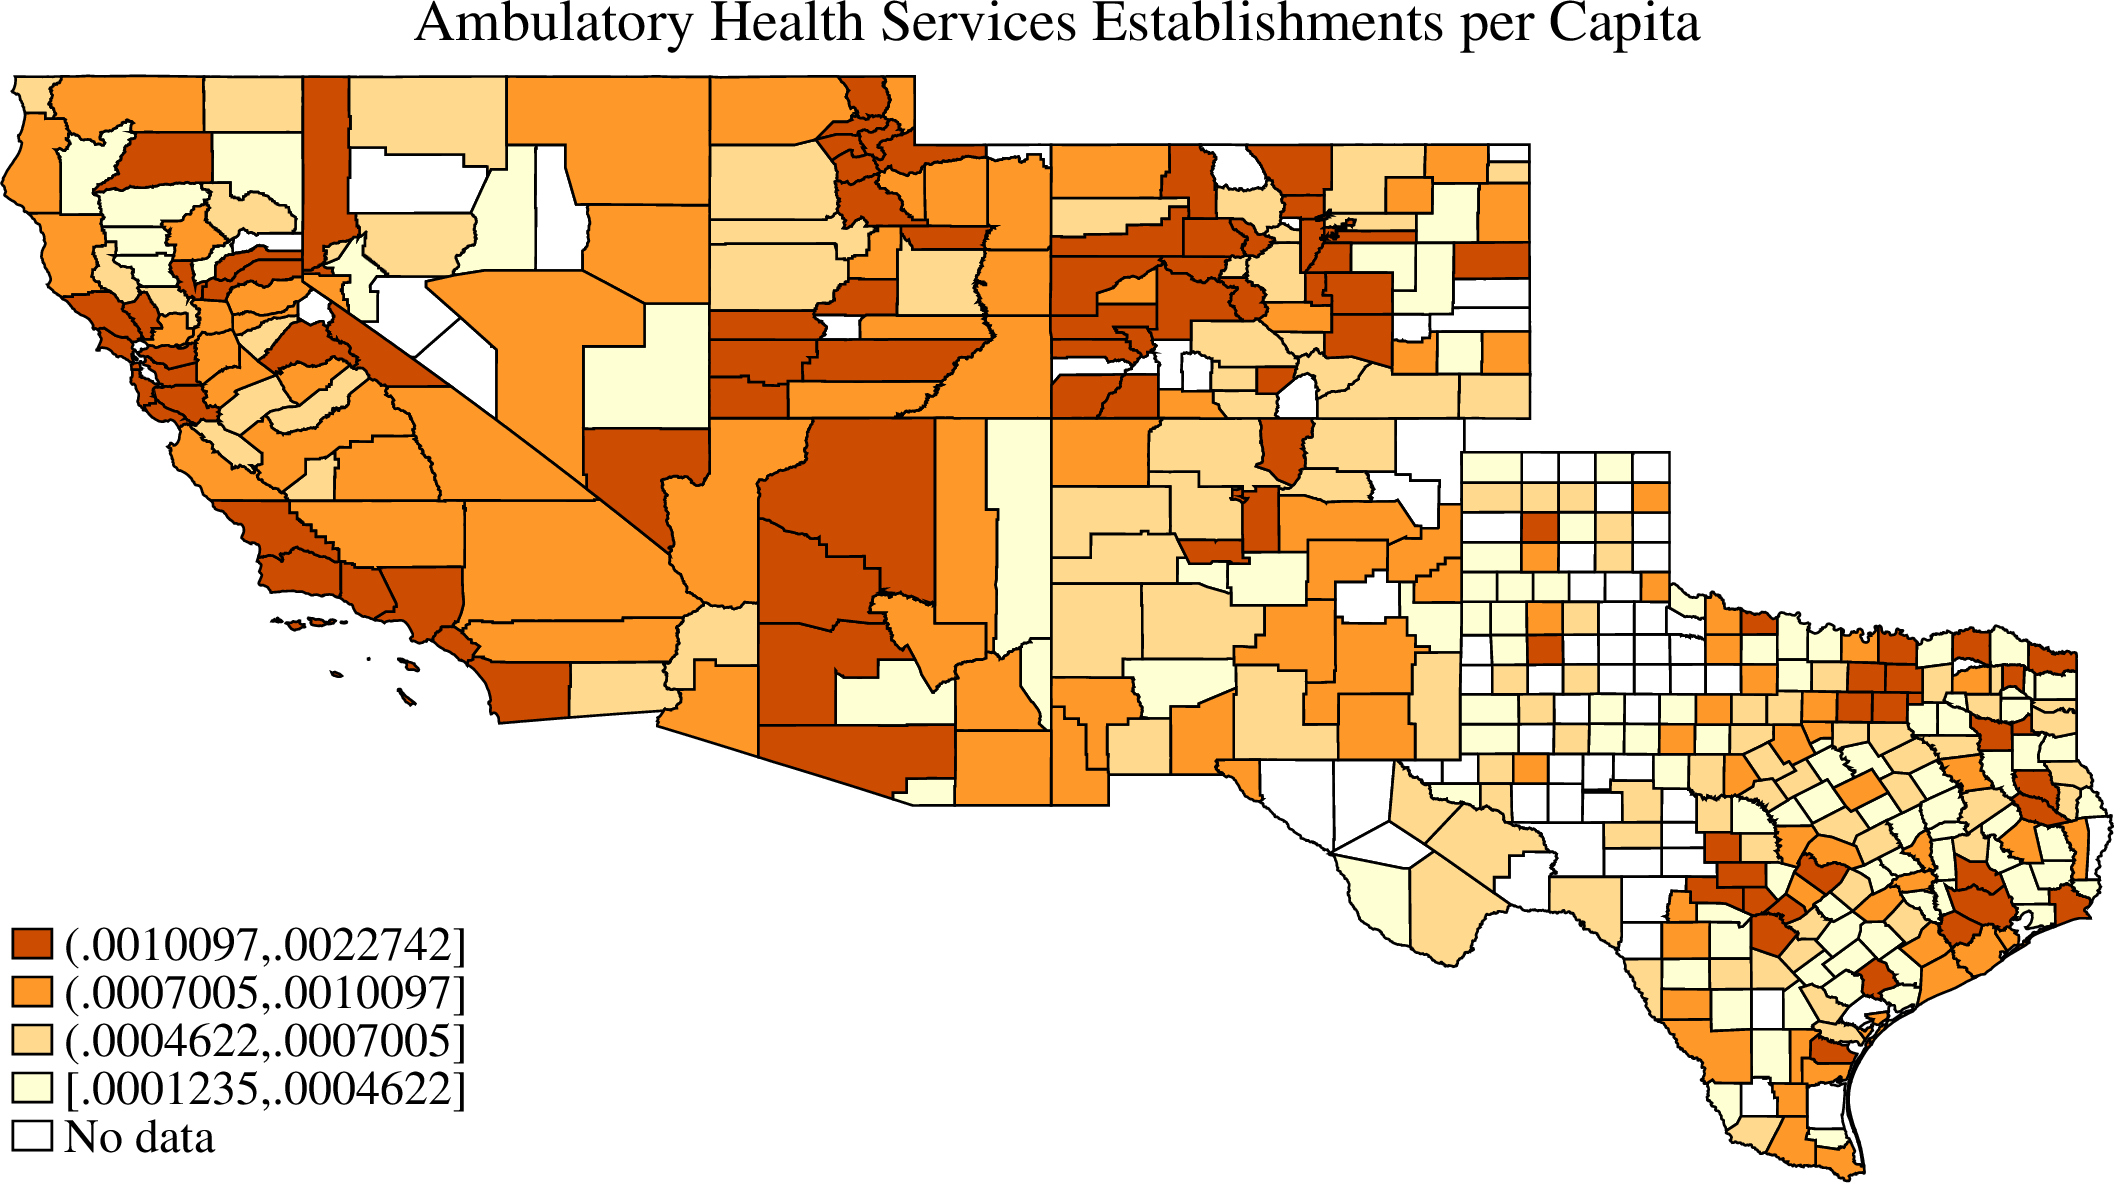
\includegraphics[width=.8\textwidth]{input/amb_health_services_estabs_pc_border.png}
\end{figure}
